\section{\textsc{Egg in a saucer}}

\subsection*{Ingredients for 2 bowls:}

\begin{tabular}{p{7.5cm} p{7.5cm}}
	& \\
	2 eggs & butter to grease \\
	salt \&pepper &
\end{tabular}

\subsection*{Serving suggestion:}

%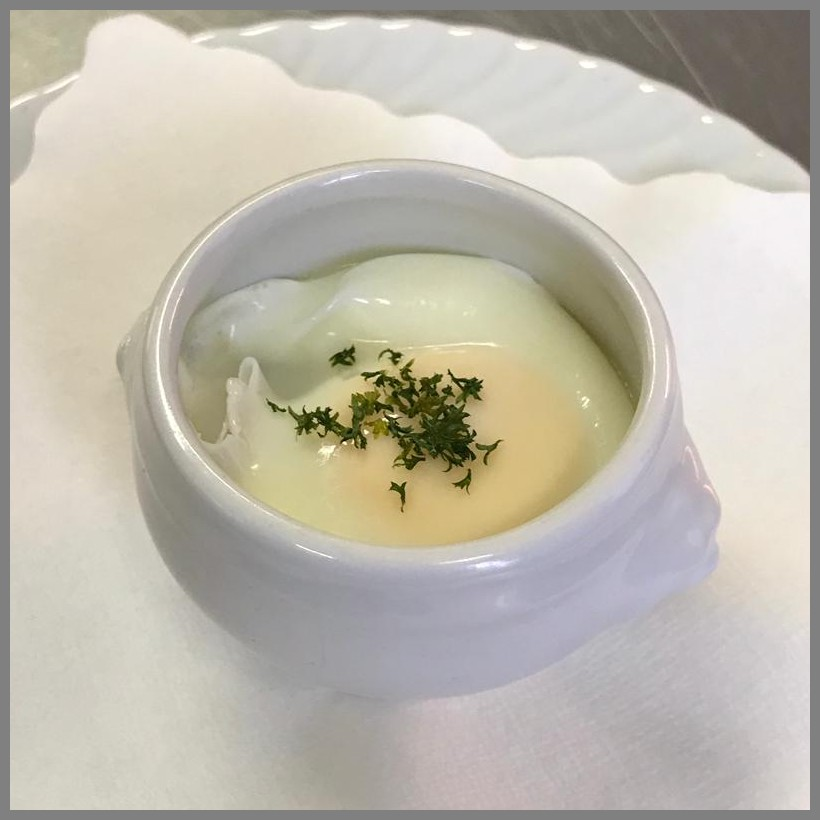
\includegraphics[width=\textwidth]{img/ei_naepfchen.jpg} \cite{eiimnaepfchen}

\subsection*{How it's done:}

\begin{tabular}{p{15cm}}
	\\
  Grease the moulds with butter. Break one egg per person into one bowl.\\
  Season with salt and pepper.\\
  Fill one pot to 1/3 with water. Bring to the boil slowly.\\
  Place the cups in the boiling water.\\
  Put the lid on the pot and cook for about 20 minutes.\\
  Carefully lift out of the pot and serve.\\
  \vspace{0.5cm}
  \textbf{Tip:} The dish can be varied according to taste. Ingredients such as cheese, bacon or onions can be added. It is also possible to “play” with the spices. Fresh herbs go perfectly with it.
\end{tabular}
